%%%%%%%%%%%%%%%%%%%%%%%%%%%%%%%%%%%%%%%%%%%%%%%%%%%%%%%%%%%%%%%%%%%%%%%%%%%%%%%%
\chapter{ПРОЕКТИРОВАНИЕ АРХИТЕКТУРЫ МОДУЛЯ SIP-ТЕЛЕФОНИИ}
%%%%%%%%%%%%%%%%%%%%%%%%%%%%%%%%%%%%%%%%%%%%%%%%%%%%%%%%%%%%%%%%%%%%%%%%%%%%%%%%

Перед разработкой, необходимо обдумать на каком уровне находится разрабатываемый модуль SIP-телефонии по отношению к элементам браузера и web-приложению. Так же необходимо определить основные части модуля и его архитектуру.

\section{Взаимодействие браузера, модуля SIP-телефонии и web-приложения}

\begin{figure}[h!]
\center{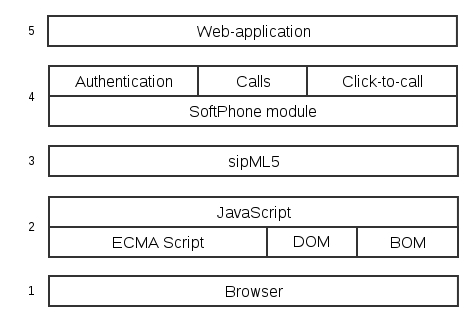
\includegraphics[width=0.75\linewidth]{modulesStructure}}
\caption{Взаимодействие браузера, модуля SIP-телефонии и web-приложения}
\label{image:modulesStructure}
\end{figure}

На рисунке \ref{image:modulesStructure} изображена взаимодействие браузера, модуля SIP-телефонии и web-приложения. Поясним назначение каждого уровня:

\begin{enumerate}
\item На этом уровне расположены следующие компоненты браузера: объектная модель документа (Document Object Module, DOM), объектная модель браузера (Browser Object Module, BOM) и WebRTC. Объектная модель документа может хранить такие элементы как аудио, которые позволят нашему модулю воспроизводить рингтон и звук гудков. WebRTC предоставляет возможность захватывать аудио с микрофона, кодировать его, и передавать при помощи WebSockets. При приёме аудио WebRTC предоставляет возможность фильтровать его алгоритмами VoIP-телефонии.

\item Данный уровень представляют функции JavaScript, которые реализуют доступ web-страницы к элементам объектной модели документа и WebRTC.

\item На этом уровне располагается выбранная нами библиотека sipML5. Она обеспечивает обмен аудио-данными по протоколу SIP. То есть анализирует пакеты приходящие от WebSockets и если они являются SIP-пакетами, то поступают на обработку.

\item Этот уровень является основной частью разработки. Здесь должны быть реализованы функции, которые легко использовать для звонка. Эти функции будут вызываться SIP-событиями, или по инициативе пользователя, и будут являться обёртками для библиотеки sipML5.

Здесь же необходимо реализовать интерфейс взаимодействия с web-приложением. Основными функциями этого интерфейса будут являться: получение данных о SIP-аккаунте (Аuthentication), оповещения о звонке (Calls), и функция click-to-call, которая при нажатии на номер телефона в web-приложении набирает его.

\item На верхнем модуле располагается web-приложение, которое будет подключать разрабатываемый нами модуль как файл на JavaScript.
\end{enumerate}

\section{Архитектура модуля SIP-телефонии}

На рисунке \ref{image:architecture} изображена архитектура модуля. Опишем каждую его часть.

\begin{figure}[h!]
\center{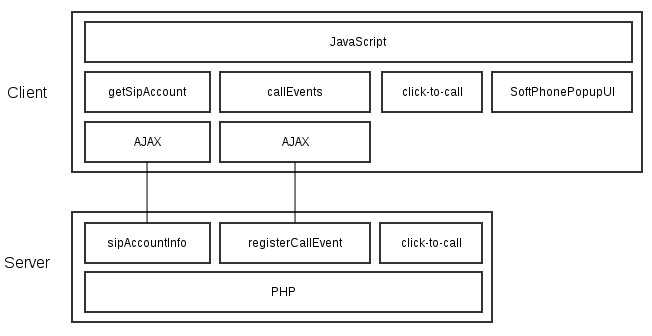
\includegraphics[width=0.9\linewidth]{architecture}}
\caption{Архитектура модуля}
\label{image:architecture}
\end{figure}

Основой модуля является его ядро softPhoneJS. Оно обеспечивает взаимодействие с библиотекой sipML5 и отслеживает состояние звонка.

При переключении состояния звонка информация передаётся в модуль CallEvents, который отправляет информацию на сервер, для регистрации звонка. Для передачи данных в этом случае проще всего использовать AJAX.

Однако перед тем как звонить, необходимо получить из web-приложения данные о SIP-аккаунте. За это отвечает модуль getSipAccount. Данные так же передаются при помощи AJAX.

SoftPhonePopupUI отвечает за графический интерфейс скользящей кнопки и плавающего окна. Должны быть реализованы функции, которые обрабатывают перетаскивание окна мышью.

\begin{figure}[h!]
\center{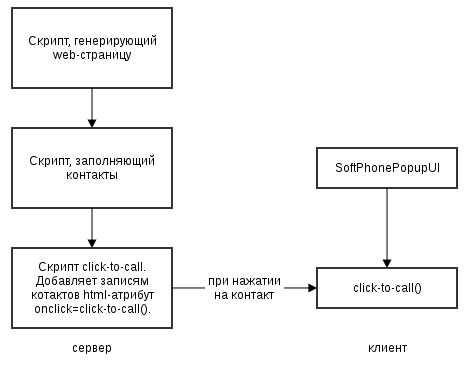
\includegraphics[width=0.75\linewidth]{ClickToCall}}
\caption{Реализация click-to-call}
\label{image:ClickToCall}
\end{figure}

Click-to-call сам набирает номер при нажатии на контакт. Однако в этом случае обмен происходит не через AJAX. Реализация функции click-to-call изображена на рисунке \ref{image:ClickToCall}.

Скрипт, генерирующий web-страницу заполняет её контактами, но перед этим добавляет каждому контакту html-атрибут, который вызывает функцию обработчика при клике по контакту. Обработчиком задаётся функция click-to-call которая реализована на клиенте в модуле SoftPhonePopupUI.

\section{Резюме}

В данном разделе была рассмотренна иерархия web-приложения, определено какое место занимает модуль SIP-телефонии, встроенный в него. Выделены основные части модуля SIP-телефонии, разработана его архитектура, выбраны способы взаимодействия с сервером.
